\begin{figure}
    \centering
    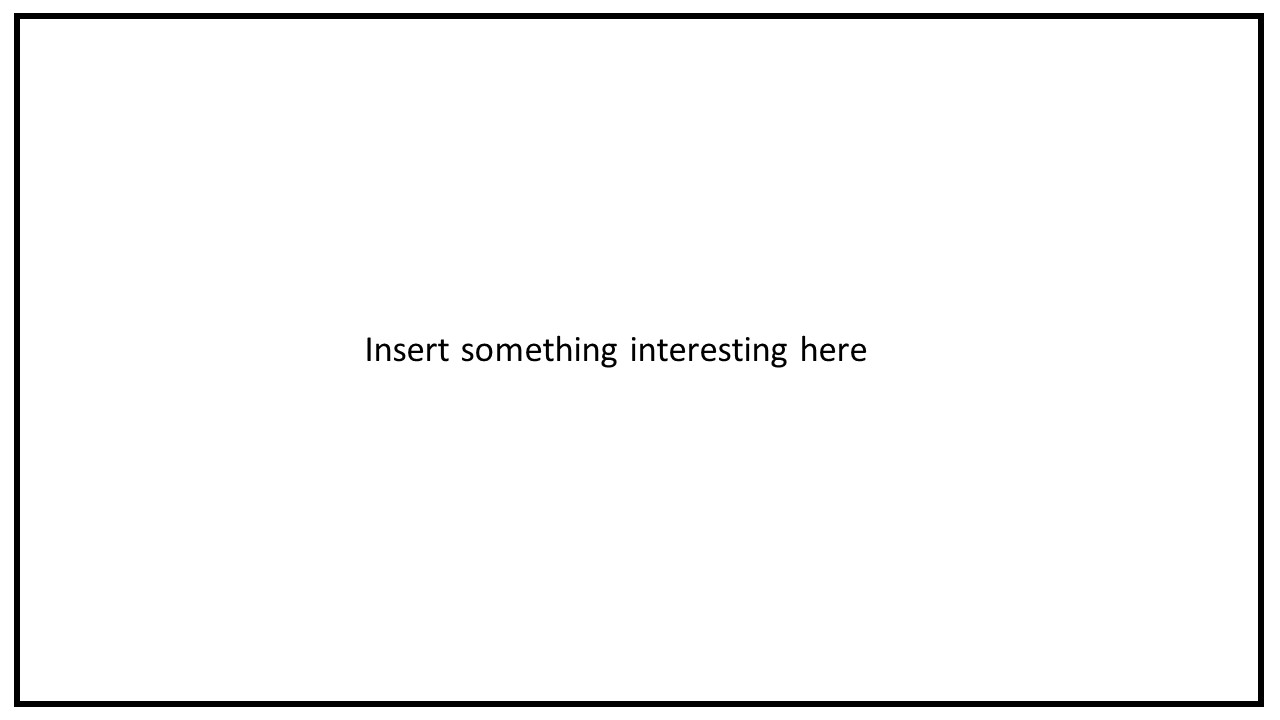
\includegraphics[width=0.98\linewidth]{Other/empty.jpg}
    \caption[Figure that shows how the HWP improves sensitivity and/or systematics]{Figure that shows how the HWP improves sensitivity and/or systematics}
    \label{fig:hwp_systematics}
\end{figure}

\begin{figure}
    \centering
    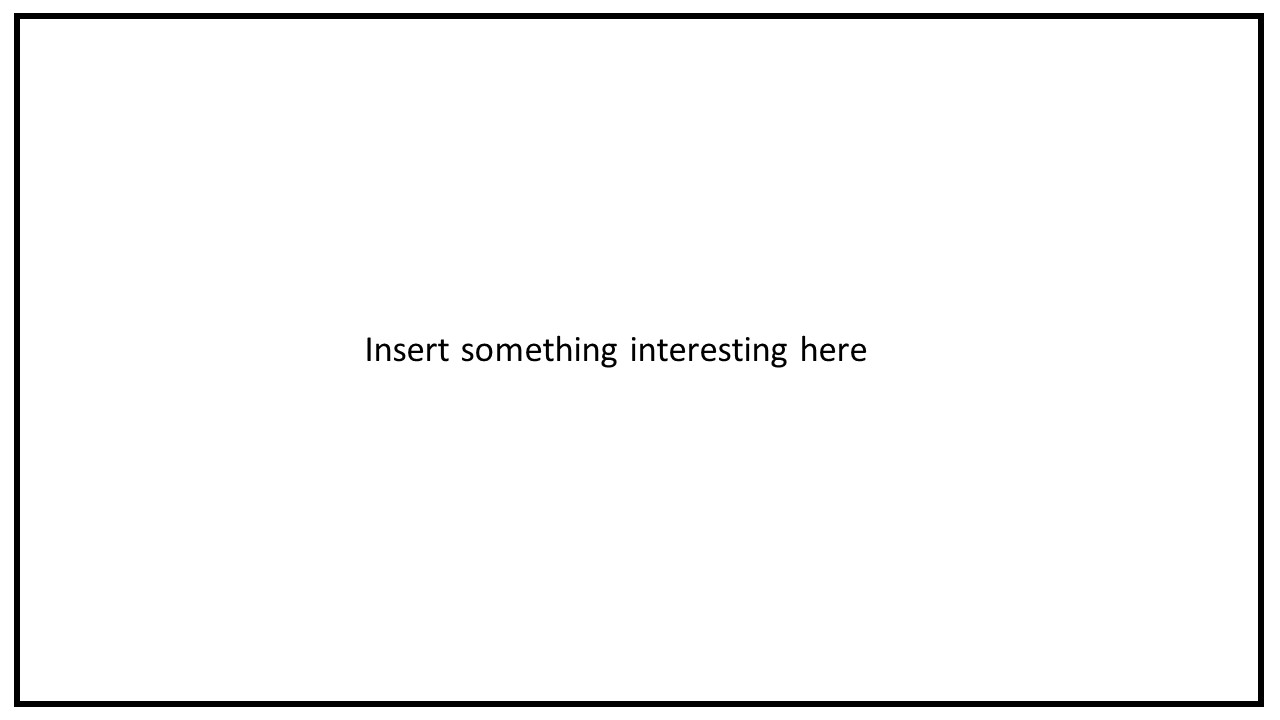
\includegraphics[width=0.98\linewidth]{Other/empty.jpg}
    \caption[Poincare sphere depiction of acrhomatic HWP operation]{Poincare sphere depiction of acrhomatic HWP operation}
    \label{fig:poincarel}
\end{figure}

=  \left< \left| E_{a} \right|^{2} \right> + \left< \left| E_{b} \right|^{2} \right> = \left< \left| E_{l} \right|^{2} \right> + \left< \left| E_{r} \right|^{2} \right>

The second and most relevant HWP demonstration to this dissertation is that of the POLARBEAR experiment. POLARBEAR was not originally designed to use a continuously rotating HWP, but after its successes measuring lensing B-modes during its first two observation seasons, the POLARBEAR team retrofitted a HWP to the existing system to enable the pursuit of primordial B-modes. The POLARBEAR telescope design is virtually equivalent to that of SA, and its receiver contains 150~GHz TES bolometers and a Lyot stop that defines a $\sim$~3~arcmin resolution on the sky. POLARBEAR installed the HWP at \important{prime focus}, which is at the focal plane of the primary mirror, located between the primary and secondary mirrors. Therefore, like that of ABS, the POLARBEAR HWP operates at ambient temperature, but unlike that of ABS, it is not the first optical element in the telescope system. This second feature introduces unique analysis challenges that prompted innovative data processing techniques in the drive for a low $\ell_{\mathrm{knee}}$ using a high-angular-resolution telescope.

%%%%%%%%%%%%%%%%%%%%%%%%%%%%%%%%
%%%%%%%%%%%%%%%%%%%%%%%%%%%%%%%%

\section{Precedent}
\label{sec:hwp_precedent}

Given the motivations for deploying a HWP and a description of its basic operation, we now have a foundation upon which to present the SA HWP mechanisms described in Chapters~blah and~blah. However, before diving into those specific applications, we want to provide a brief overview of the precedent for operating a HWP modulator at the Atacama sight. Much of the modulator research in this thesis stands on the shoulders of previous HWP demonstrations, and we will highlight two of those demonstrations here.

The Atacama B-mode Search (ABS) was a small aperture telescope that observed from the Atacama site from 2012 - 204. It used TES bolometers observing at 150~GHz, and it used a continuously rotating HWP as its first optical element to modulate sky polarization. While ABS had a large NET and therefore was unable to make set a competitive constraint on the tensor-to-scalar ratio, the HWP was quite effective at suppressing 1/f noise in its demodulated data and as a result achieved a 1/f knee  of $\sim$~1~mHz. ABS's temporal power spectra before and after HWP demodulation are shown in Figure~blah, and the level of atmospheric 1/f rejection is quite substantial. In addition, the ABS team studied their telescope beam using planets as point sources to map the far-field optical response. Using the same monopole/dipole/quadrupole decomposition discussed in Section~\ref{sec:polarized_beam_systematics}, they found polarization leakage to be well controlled, further emphasizing the HWP's viability as a systematic mitigator. The ABS demonstration was seminal for the prospect of low-$\ell$ science at the Atacama site, and it has inspired further waveplate development for other experiments on the Chajnantor Plateau.